\documentclass{beamer}
%\documentclass[handout]{beamer}
%\documentclass[handout, notes=show]{beamer}

\usepackage[french]{babel}
\usepackage[utf8]{inputenc}
\usepackage{times}
\usepackage[T1]{fontenc}

\usepackage{graphicx}
\graphicspath{{../report/img/}{./img/}}
\usepackage{hyperref}
\hypersetup{colorlinks=true,linkcolor=red}
\usepackage{pgfpages}

\mode<presentation>
{
    \useinnertheme[shadow]{rounded}
    \useoutertheme{default}
    \usecolortheme{lily}
    \usecolortheme{whale}
    \usecolortheme[named=darkgray]{structure}

    \beamertemplatenavigationsymbolsempty
    \setbeamercovered{transparent=10}
    \setbeamertemplate{footline}
    {
        \hfill \footnotesize{\insertframenumber/\inserttotalframenumber} \hspace{0.5cm}
        \vspace{0.5cm}
    }
}

\title[]{Mathématiques discrètes}
\subtitle{Blackjack}
\author{Claudio Sousa, David Gonzalez}
\institute{HEPIA}
\date{21/06/2018}

\pgfdeclareimage[width=1cm]{logo}{logo}
\logo{\pgfuseimage{logo}}

\setcounter{tocdepth}{3}

\begin{document}

\begin{frame}[plain]
    \titlepage
\end{frame}

\section{Catégorisation}

\begin{frame}
    \frametitle{Catégorisation}
    \begin{itemize}
        \item Mouvements (coups) séquentiels
        \item Partie itératifs
        \item Avec somme nulle
        \item Avec information partielle
        \item Aléatoire
        \item Compétitif
    \end{itemize}
\end{frame}

\section{Tests empiriques}

\begin{frame}
    \frametitle{Tests empiriques: Chance du joueur avec stratégie basique}
    \begin{figure}[H]
        \begin{center}
            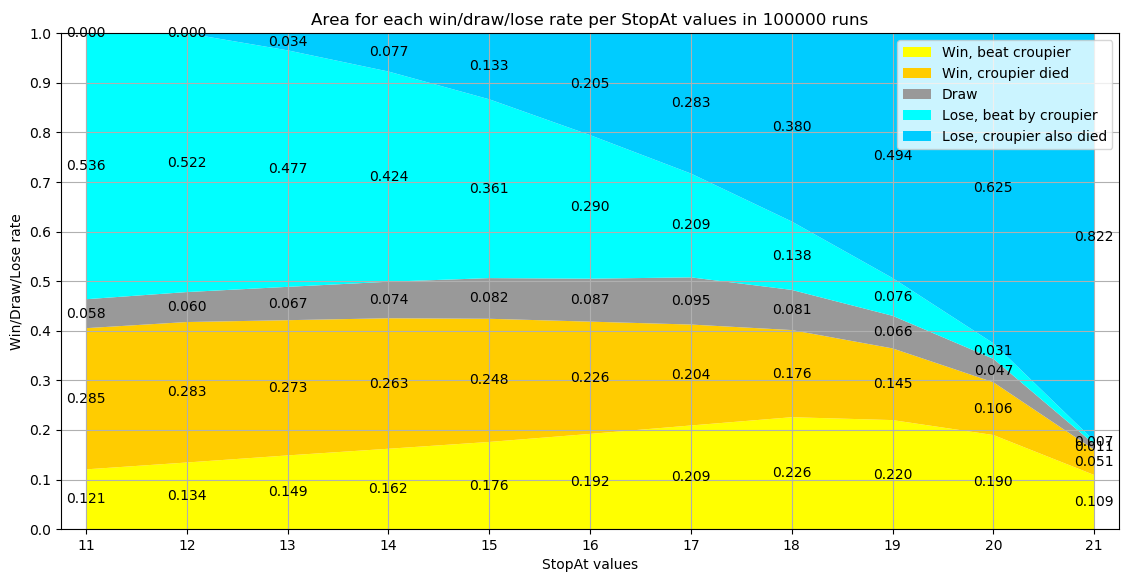
\includegraphics[width=1\textwidth]{empirical_graph1}
        \end{center}
    \end{figure}
\end{frame}

\begin{frame}
    \frametitle{Tests empiriques: Chance du joueur par main initial du croupier}
    \begin{figure}[H]
        \begin{center}
            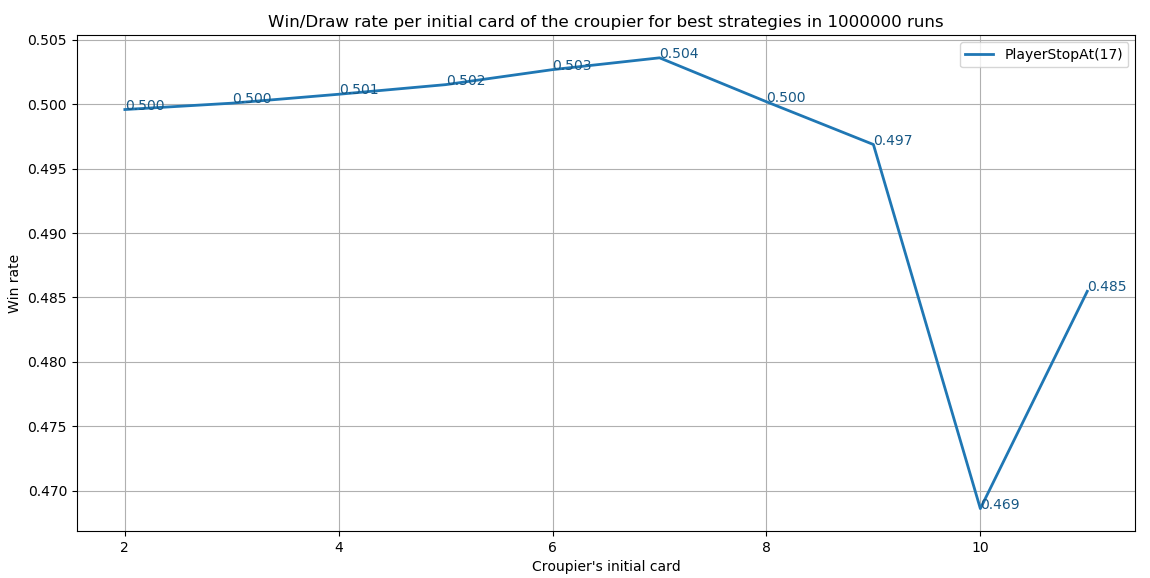
\includegraphics[width=1\textwidth]{empirical_graph2}
        \end{center}
    \end{figure}
\end{frame}

\begin{frame}
    \frametitle{Tests empiriques: Comparaison de stratégies}
    \begin{figure}[H]
        \begin{center}
            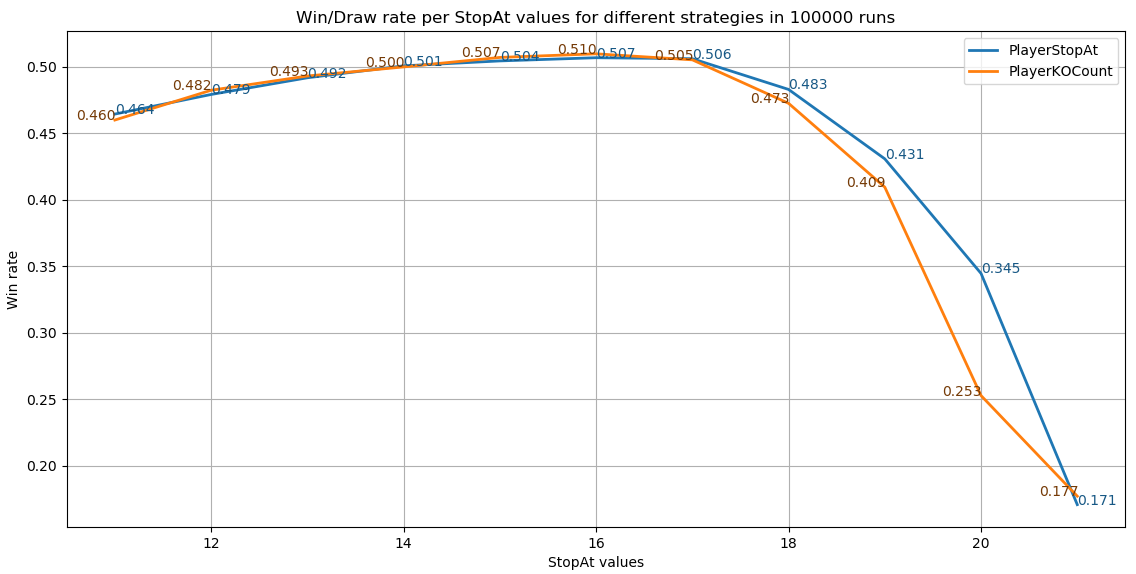
\includegraphics[width=1\textwidth]{empirical_graph3}
        \end{center}
    \end{figure}
\end{frame}

\section{Théorie}

\begin{frame}
    \frametitle{Théorie: Chance du croupier}
    \begin{figure}[H]
        \begin{center}
            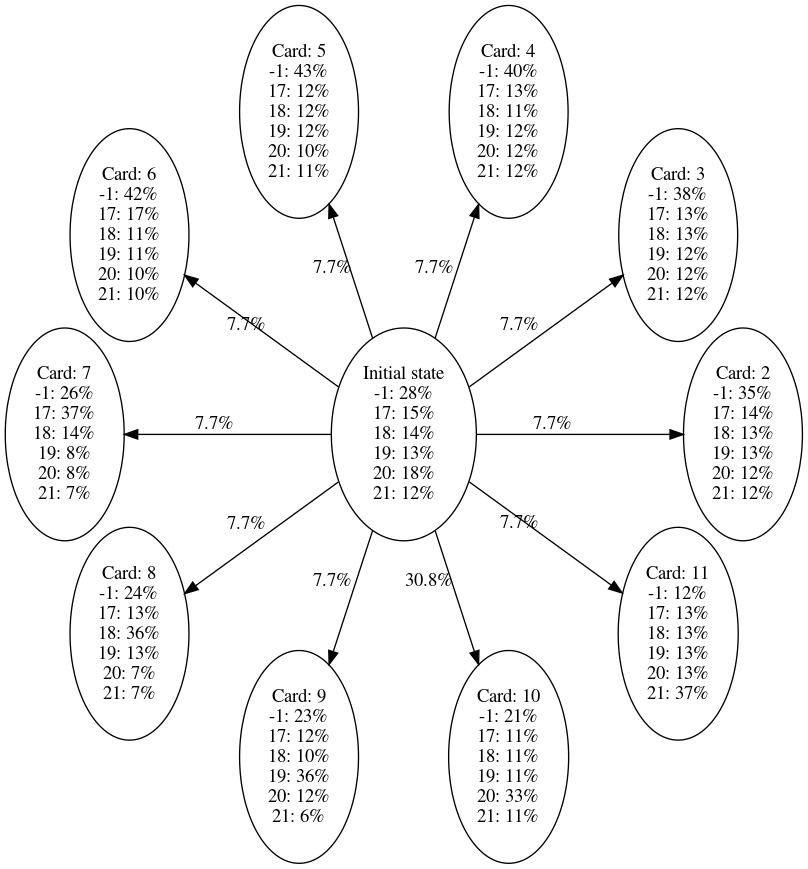
\includegraphics[width=0.7\textwidth]{theoretical_croupier}
        \end{center}
    \end{figure}
\end{frame}

\begin{frame}
    \frametitle{Théorie: Chance du joueur}
    \begin{figure}[H]
        \begin{center}
            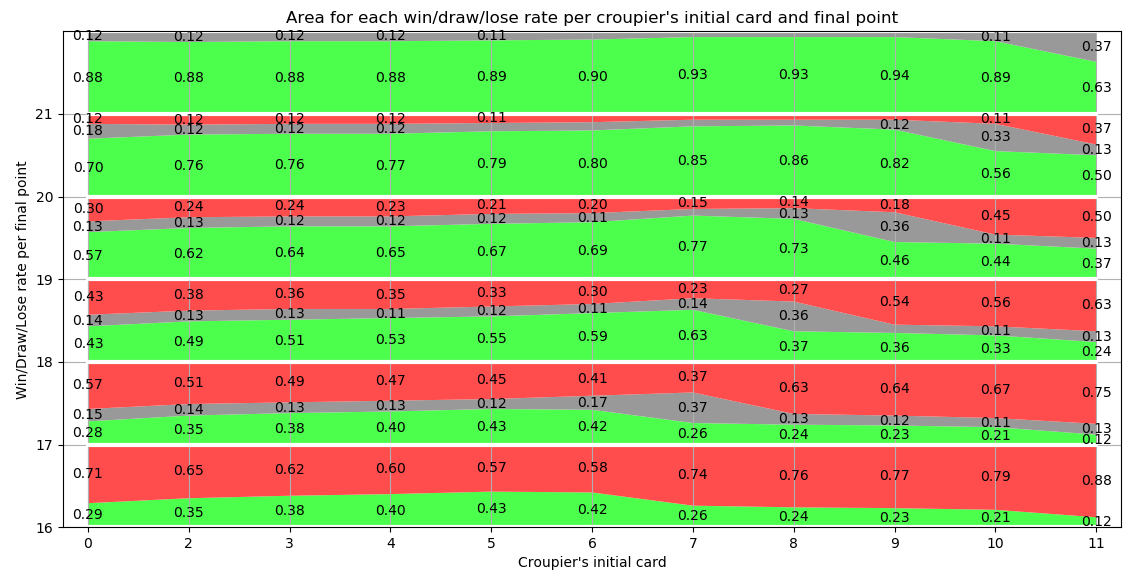
\includegraphics[width=1\textwidth]{theoretical_graph1}
        \end{center}
    \end{figure}
\end{frame}

\end{document}
